\documentclass[addpoints]{exam}

\printanswers
\bracketedpoints

\usepackage{amsmath}
\usepackage{amssymb}
\usepackage{graphicx}
\usepackage{color}



\footer{ELE6209A}{Page \thepage\ de \numpages}{Été 2022}

%\input{commands.tex}

\begin{document}

\begin{coverpages}
\coverfooter{ELE6209A}{Page de couverture}{Été 2022}

%\title{Examen Final\\ ELE3202 - Introduction \`a l'automatisation\\
%\vspace{0.5cm}
%\large D\'epartement de g\'enie \'eletrique\\\'Ecole Polytechnique de Montr\'eal}
%\date{Vendredi 19 avril 2013\\
%\vspace{0.2cm}
%Dur\'ee: 2h30, de 13h30 \`a 16h00}
%\maketitle

\begin{center}
\makebox[\textwidth]{\Large{ELE6209A - Systèmes de navigation}} 
\vspace{0.5cm}

\makebox[\textwidth]{\large{Département d'ingénierie électrique}}

\makebox[\textwidth]{\large{\'Ecole Polytechnique de Montr\'eal}}

\vspace{0.5cm}
\makebox[\textwidth]{\large{Été 2022}}


\end{center}

\begin{center}
\makebox[\textwidth]{Instructor: J\'er\^ome Le Ny} \\ %, \textbf{poste 4886}} \\
\vspace{0.5cm}
\fbox{\fbox{\parbox{5.5in}{\centering
Answer the questions on the exam book. \\%R\'epondre aux questions sur le cahier d'examen distribu\'e. \\
Always clearly and concisely explain the reasoning leading to your answers. Numerical answers without
explanations can be counted as wrong, even if the result is correct. \\ %Expliquer clairement votre raisonnement pour arriver \`a vos r\'eponses. \\
Your answers can be written in English or French. \\%Les r\'eponses peuvent \^etre r\'edig\'ees en fran\c{c}ais ou en anglais.\\
You do not have to answer the problems in the order provided. However, you must group your answers
to the questions of the same problem together. \\
If relevant, the units in which your numerical answers are expressed must be stated.
Manage your time carefully: the points attributed to each question should give you an indication on how much
time to spend on them. Not all questions are of the same difficulty. I recommend you first skim through the exam
to identify the problems you are most comfortable with. \\ 
\vspace{0.5cm}
Documents allowed: instructor's lecture notes and slides. \\%Une calculatrice non programmable est permise.
A non-programmable calculator is allowed. \\
Please return the question sheet at the end.
}}}
\end{center}

\vspace{2cm}
\begin{center}
\textcolor{red}{\textbf{SOLUTION}}
\end{center}

\vspace{3cm}
\begin{center}
\gradetable[h][questions]
\end{center}


\newpage
\begin{center}
- This page intentionally left blank -
\end{center}

\end{coverpages}





%%%%%%%%%%%%%%
% Start of the exam
%%%%%%%%%%%%%%


\begin{questions}

\question
\begin{parts}
\part[2]  Si \{b\} correspond au repère attaché à un véhicule et \{n\} représente le repère de navigation NED centré au centre de masse du véhicule. En se basant uniquement sur les mesures d'un magnétomètre ainsi qu'un accéléromètre, trouver la matrice de rotation $R^b_n$.

\part[2] Décortiquer le fichier $magneto\_accel\_measurements.csv$. Utiliser le langage de votre choix. Donner le graphique des angles eulers en degré, $[\phi,\theta,\psi]$ pour tout l'interval de temps. Utiliser la convention XYZ. Vous pouvez utiliser le fichier $quaternionRef.csv$ afin de vérifier votre réponse.

\end{parts}


\begin{solution}
\begin{parts}

\part On pose que le magnétomètre $m = [m_x,m_y,m_z]^T$ et l'acéléromètre $a = [a_x,a_y,a_z]^T$.

\begin{equation}
    R^b_n = DCM = \begin{bmatrix} N & E & D\end{bmatrix} = \begin{bmatrix} m & -a\times m & -a\end{bmatrix}
\end{equation}

\part

$\psi$ = rotation autour de l'axe Z\\
$\theta$ = rotation autour de l'axe Y\\
$\phi$ = rotation autour de l'axe X\\

La rotation finale est :
\begin{align}
    \nonumber\psi = 30\\
    \nonumber\theta = -50\\
    \nonumber\phi = 90   
\end{align}

Voici le graphique représentant les rotations en degré dans le temps:

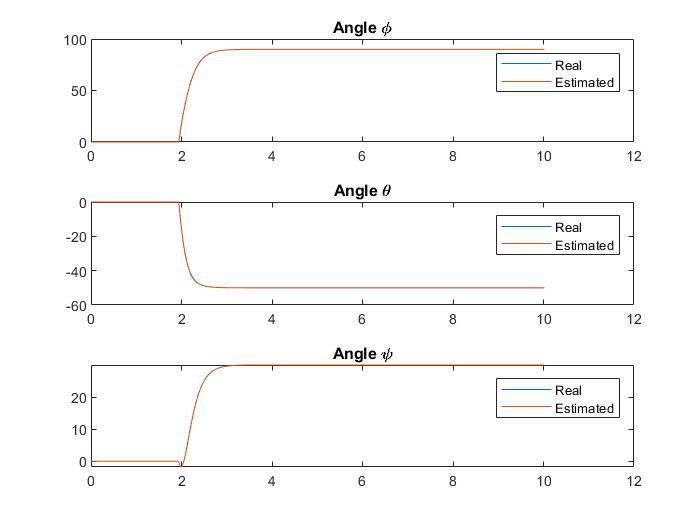
\includegraphics[width=0.8\textwidth]{image/Q1_b.JPG}

\end{parts}
\end{solution}

\question[4]
En utilisant les données du fichier $gyroData.csv$ intégrer les données du gyroscope sur la période complète. Vous pouvez assumer que la rotation initiale de l'objet est 0. Donner le graphique des angles eulers en degré, $[\phi,\theta,\psi]$ pour tout l'interval de temps. Utiliser la convention XYZ. Vous pouvez utiliser le fichier $quaternionRef.csv$ afin de vérifier votre réponse. Utiliser le langage de votre choix.

\begin{solution}
    L'intégration de Poisson est utilisée.\\
    $\psi$ = rotation autour de l'axe Z\\
    $\theta$ = rotation autour de l'axe Y\\
    $\phi$ = rotation autour de l'axe X\\
     Voici le graphique représentant les rotations en degré dans le temps:
    
    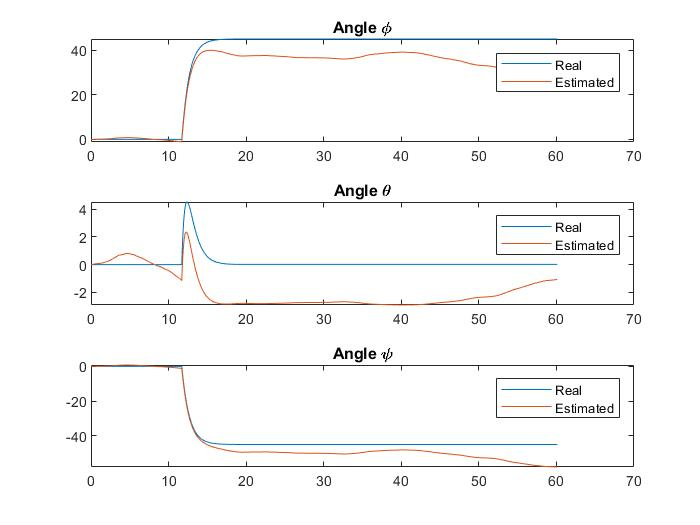
\includegraphics[width=1\textwidth]{image/Q2.JPG}
\end{solution}

\question Dans le langage de votre choix, réaliser un filtre AHRS en se basant sur la théorie du chapitre 10. L'IMU utilisé a les erreurs suivantes:
\begin{align}
    \nonumber \nu_w &\sim \mathcal{N}(0,\,1.45\times10^{-5})\\
    \nonumber \nu_{x_w} &\sim \mathcal{N}(0,\,7.615\times10^{-4})\\
    \nonumber \nu_a &\sim \mathcal{N}(0,\,1\times10^{-5})\\
    \nonumber \nu_{x_a} &\sim \mathcal{N}(0,\,9\times10^{-5})\\
    \nonumber \nu_m &\sim \mathcal{N}(0,\,5.3\times10^{-5})\\
    \nonumber \omega^n_{n/i} &\sim \mathcal{N}(0,\,1\times10^{-5})
\end{align}

\begin{parts}
\part[8] Filtrer les données du fichier $imu\_data\_a.csv$. Vous pouvez assumer que la rotation initiale de l'objet est 0. Donner le graphique des angles eulers en degré, $[\phi,\theta,\psi]$ pour tout l'interval de temps.  Utiliser la convention XYZ. Vous pouvez utiliser le fichier $quaternionRef.csv$ afin de vérifier votre réponse.

\part[4]  Filtrer les données du fichier $imu\_data\_b.csv$. Cette fois ci  la rotation initiale de l'objet est inconnue. Il est possible de récupérer l'orientation initiale à l'aide de l'algorithme trouvé à la question 1. Donner l'orientation initiale ainsi que le graphique des angles eulers en degré, $[\phi,\theta,\psi]$ pour tout l'interval de temps.  Utiliser la convention XYZ. Vous pouvez utiliser le fichier $quaternionRef.csv$ afin de vérifier votre réponse.
\end{parts}

\begin{solution}
\begin{parts}
    \part Voici le graphique représentant les rotations en degré dans le temps:
    
    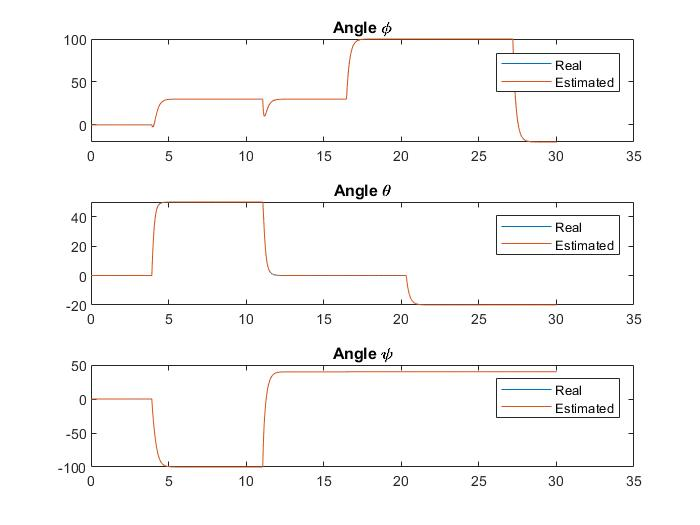
\includegraphics[width=1\textwidth]{image/Q3_a.jpg}
    
    \part Les angles initiaux sont :
    \begin{align}
        \nonumber\psi = -45\\
        \nonumber\theta = 0\\
        \nonumber\phi = 50   
    \end{align}
    
    Voici le graphique représentant les rotations en degré dans le temps:
    
    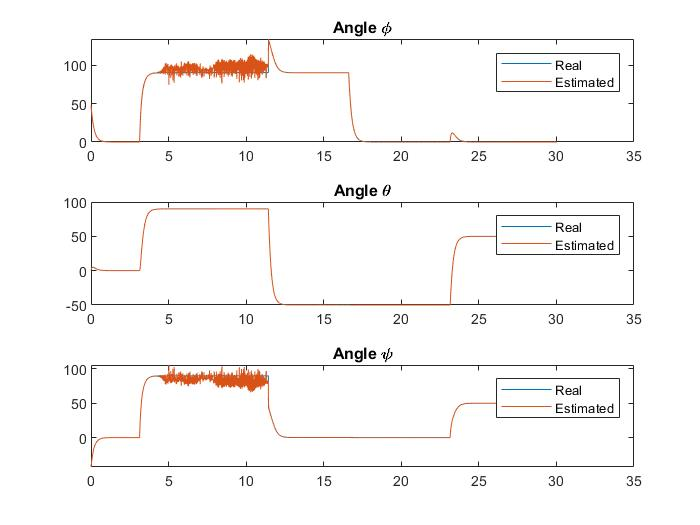
\includegraphics[width=1\textwidth]{image/Q3_b.jpg}
\end{parts}
    
\end{solution}
\end{questions}





\end{document}
